\documentclass[a4paper,10pt]{article}
\usepackage[utf8]{inputenc}
\usepackage{amstext}
\usepackage{listings}
\usepackage{graphicx}
\usepackage[T1]{fontenc}
\usepackage[utf8]{inputenc}
\usepackage[font=small,labelfont=bf]{caption}
\usepackage{float}
\usepackage[dutch]{babel}

\DeclareCaptionLabelFormat{andtable}{#1~#2  \&  \tablename~\thetable}


%opening
\title{Radio communicatie met Arduino}
\author{Patrick van Looy \& Bram Leenders}

\begin{document}

\maketitle

\section{Inleiding}
Met behulp van radiocommunicatie kunnen apparaten, zoals computers, met elkaar communiceren zonder een fysieke verbinding daarvoor nodig te hebben. Dit leent zich voor het makkelijk opzetten van (grote) netwerken, omdat de verbindingen zonder planning vooraf kunnen worden opgezet. Bij bijvoorbeeld Smart Dust kunnen de agents na de verspreiding zelf connecties opzetten en hier gebruik van maken.

Een nadeel van draadloze communicatie, is dat er vaak meer last is van storing dan wanneer er een fysieke verbinding (i.e. een kabel) aanwezig is. Doordat de communicatie niet "afgesloten" van de buitenwereld plaats vind, kunnen er externe storingszenders zijn. Voorbeelden van storingen zijn bijvoorbeeld andere agents die communiceren, obstakels die een signaal blokkeren of weerkaatsing van eerder gestuurde berichten.

Dit onderzoek kijkt naar de mogelijkheden van radiocommunicatie via Arduinos en welke rol de configuratie hierbij speelt. Allereerst wordt het onderzoeksdoel aangeduid waarna de methodes om dit doel te onderzoeken worden besproken. Vervolgens worden de resulaten gegeven en toegelicht. Als laatste wordt beschreven wat hieruit geconcludeerd kan worden en of er nog verder onderzoek gedaan kan worden.

\section{Probleemstelling}
Zoals eerder genoemd, is draadloze communicatie niet altijd even betrouwbaar. Dit wordt veroorzaakt door verschillende factoren, denk hierbij aan de keuze voor het kanaal, de omgeving, de signaalsterkte enzovoorts. In het meest optimale geval zijn er zo min mogelijk van deze belemmerende factoren aanwezig. Door deze factoren mee te nemen kijkt dit onderzoek of er een manier is waardoor draadloze communicatie zo betrouwbaar mogelijk gemaakt kan worden.

In dit onderzoek wordt gekeken naar verschillende modi waarop radiocommunicatie met Arduino's gedaan kan worden. Het doel is om erachter te komen welke modus het minst last heeft van storing en (dus) de laagste packet error rate heeft.

In de tests wordt het effect van drie verschillende factoren onderzocht:
\begin{itemize}
    \item Het frequentiekanaal
    \item De outputpower van verzonden pakketten
    \item Datatransmissiesnelheid
\end{itemize}

Bij de verschillende tests is gekeken naar het effect van verandering van de output power op de error rate. Hierbij is de hypothese dat een sterker output signaal bij de zender een sterker input signaal bij de ontvanger geeft. Dus, dat een sterker input signaal een lagere error rate geeft.

De tests moeten uitslag geven welke instellingen zorgen voor de beste communicatie.

\section{Methodologie}
Om "beste" communcatie kwantificeerbaar te maken gebruiken we de packet error rate. We defini\"eren de error rate als het aantal niet of incorrect ontvangen berichten gedeeld door het aantal verstuurde berichten;

\begin{math}
    \text{error rate} = \frac{\text{niet ontvangen}}{\text{verstuurd}} = 1 - \frac{\text{ontvangen}}{\text{verstuurd}} 
\end{math}

Voor stabiele communicatie is het van belang dat deze zo laag mogelijk, idealiter nul, is. Dit betekent dat er nauwelijks tot geen packets verloren gaan waardoor stabiele communicatie haalbaar is. In dit onderzoek is de error rate de enige eigenschap waarop we de instellingen beoordelen, en laten we andere factoren zoals bandbreedte of opgenomen vermogen achterwege.

In de testopstelling is gebruik gemaakt van twee Arduino Uno's, de Nordic nrf24l01+ radio en de RF42 library. Tenzij expliciet anders vermeld, gebruiken de radio's frequentiekanaal 0, een transmissionspeed van 250kbps en de hoogste outputpower (0 dBm). De afstand tussen beide radio's is vijf meter en er is sprake van een line of sight (geen blokkerende objecten). De tests zijn uitgevoerd in een ruimte met andere elektrische aparatuur die ook van radiocommunicatie gebruik maakte.

Tijdens de test zendt een Arduino duizend maal een pakket; wanneer de andere Arduino het pakket ontvangt stuurt deze hem terug. Wanneer het pakket voor de tweede maal ontvangen wordt, telt dat als \'e\'en succesvol ontvangen pakket. Er wordt dus naar een volledige roundtrip gekeken. Beide radio zenders gebruiken telkens dezelfde instellingen, en de timeout tijd is zeer ruim gekozen om dit geen beperking te laten zijn.

De gebruikte code is te zien in Appendix~\ref{sec:code}.

\section{Resultaten\&Analyse}
Deze sectie geeft de resultaten van de uitgevoerde tests en toelichting daarbij. Er zijn drie factoren onderzocht; de outputpower, het frequentiekanaal en de datatransmissiesnelheid.

\subsection{Outputpower}
In de resultaten is duidelijk terug te zien dat de eerder genoemde hypothese klopt: een sterker output signaal geeft een lagere error rate. Er is een zeer significant verschil; een toename van factor $64$ in vermogen geeft een error rate die ongeveer een factor $55$ lager is.

\begin{figure}[h!]
    \begin{minipage}{\textwidth}
        \begin{minipage}{0.49\textwidth}
            \centering
            \begin{tabular}{cc}\hline
                Outputpower &  Error rate   \\ \hline
                0 dBm       &  0.4\%        \\
                -6 dBm      &  4.8\%        \\
                -12 dBm     &  11.1\%       \\
                -18 dBm     &  21.9\%	\\ \hline
            \end{tabular}
        \end{minipage}
        \hfill
        \begin{minipage}{0.49\textwidth}
            \centering
            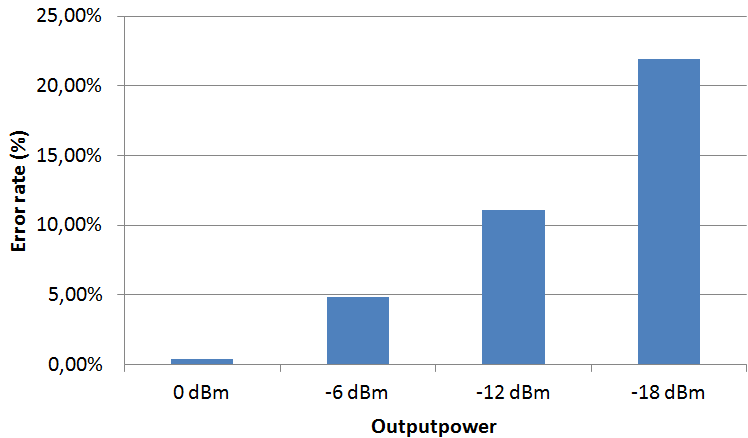
\includegraphics[width=0.9\textwidth]{outputpower.png}
        \end{minipage}
        \caption{Error rate bij verschillende output sterktes.}
    \end{minipage}
\end{figure}

\subsection{Datatransmissiesnelheid}
\begin{figure}[h!]
    \begin{minipage}{\textwidth}
        \begin{minipage}{0.49\textwidth}
            \centering
            \begin{tabular}{cc} \hline
                Datatransmissiesnelheid &  Error rate   \\ \hline
                250 kbps                &  0.4\%        \\
                1 mbps                  &  0.6\%        \\
                2 mbps                  &  0.8\%        \\ \hline
            \end{tabular}
        \end{minipage}
        \hfill
        \begin{minipage}{0.49\textwidth}
            \centering
            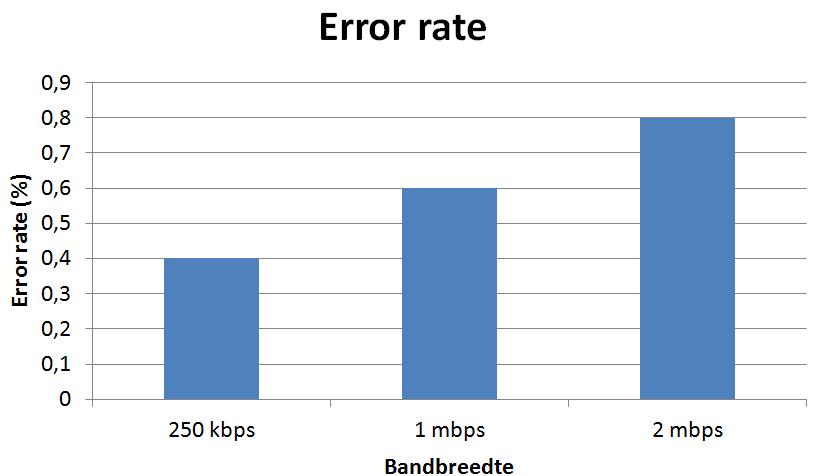
\includegraphics[width=0.9\textwidth]{bandbreedte.png}
        \end{minipage}
        \caption{Error rate bij verschillende datatransmissie snelheden.}
    \end{minipage}
\end{figure}
Bij het testen van verschillende datatransmissiesnelheden zien we dat de packet error rate slechts weinig verandert; hoewel het relatieve verschil vrij groot is (factor twee) blijft de error rate erg laag. Afgaande op deze resultaten kunnen we dus stellen dat een lage datatransmissiesnelheid de error rate positief be\"invloed.

Echter, omdat de error rate in alle gevallen erg laag was, raden we aan om eerst uitvoeriger te testen binnen opstellingen die een hogere error rate hebben.

\subsection{Frequentiekanaal}
Zoals in de introductie al kort genoemd is, kunnen radiozenders elkaar storen omdat ze hetzelfde medium gebruiken. Om dit te voorkomen kunnen zenders verschillende frequenties gebruiken, waardoor ze elkaar niet of minder storen. In de gebruikte testruimte zijn mogelijke stoorzenders onder andere omringende Arduino's en laptops die WiFi gebruiken. Omdat de frequentieband van de Arduino's (2.4 GHz) gedeeld wordt met WiFi, verwachten we dat de frequenties rond WiFi erg veel last hiervan hebben.

De testresultaten ondersteunen deze hypothese: er is duidelijk zichtbaar dat frequenties dicht bij de 2.4 GHz erg veel storing (bijna 25\%) hebben, terwijl frequenties die daar verder vanaf liggen vrijwel geen storing (1.3\% error rate) hebben. Wat verder opvalt, is dat niet alleen het precieze WiFi frequentiekanaal gestoord worden maar de frequentiekanalen ernaast ook. Het is dus zaak om een frequentiekanaal te zoeken dat zo ver mogelijk van gebruikte kanalen af ligt.

Figuur~\ref{fig:freqkanaal_table} toont een overzicht van de meetresultaten van de geteste frequentiekanalen.

\begin{figure}[h!]
    \begin{minipage}{\textwidth}
        \begin{minipage}{0.49\textwidth}
            \centering
            \begin{tabular}{cc} \hline
                Frequentiekanaal    &  Error rate   \\ \hline
                0                   &  4.7\%        \\
                15                  &  2.4\%        \\
                30                  &  10.6\%       \\
                45                  &  21.1\%       \\
                60                  &  24.6\%       \\
                75                  &  13.6\%       \\
                90                  &  1.6\%        \\
                105                 &  1.3\%        \\ \hline
            \end{tabular}
        \end{minipage}
        \hfill
        \begin{minipage}{0.49\textwidth}
            \centering
            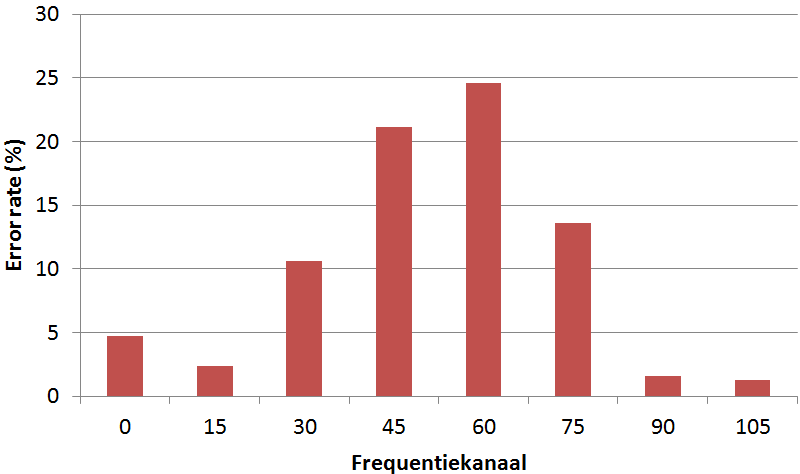
\includegraphics[width=0.9\textwidth]{frequentiekanaal.png}
        \end{minipage}
        \caption{Error rate bij verschillende frequentiekanalen.}
        \label{fig:freqkanaal_table}
    \end{minipage}
\end{figure}

\section{Conclusie}
Draadloze communicatie is niet altijd even betrouwbaar. Dit heeft verschillende oorzaken. Echter, kunnen we deze oorzaken zo'n klein mogelijke invloed geven waardoor draadloze communicatie nagenoeg stabiel plaats kan vinden?

Door de configuratie zo optimaal mogelijk te maken is uit de tests is gebleken dat de laagste packet error rate behaald wordt bij een sterk outputsignaal met lage datatransmissiesnelheid, op een frequentiekanaal dat niet door andere zenders gebruikt wordt.

Dus het is wel degelijk mogelijk om draadloze communicatie stabiel te maken door de configuratie op een dusdanige manier aan te passen dat het op de bestemde locatie naar tevredenheid functioneert.

Verder onderzoek zou nog gedaan kunnen worden naar het energieverbuik bij de verschillende instellingen. Bij dit onderzoek is dat achter wegen gelaten. Voor sommige toepassingen, zoals in sensornetwerken, zou laag energieverbruik gewenst kunnen zijn.

\newpage
\appendix
\section{Bijlage 1 - Code}
\label{sec:code}
% xxxxxxxxxxxxxxxxxxxxxxxxx Code Snippet STARTS xxxxxxxxxxxxxxxxxxxxxx
\lstset{
  language=C,                     % choose the language of the code
  stepnumber=1,                   % the step between two line-numbers. If it's 1, each line will be numbered
  basicstyle=\footnotesize,
 % numbersep=5pt,                 % how far the line-numbers are from the code
%  backgroundcolor=\color{white}, % choose the background color. You must add \usepackage{color}
  showspaces=false,               % show spaces adding particular underscores
  showstringspaces=false,         % underline spaces within strings
  showtabs=false,                 % show tabs within strings adding particular underscores
  tabsize=4,                      % sets default tabsize to 2 spaces
  captionpos=t,                   % sets the caption-position to top
  breaklines=true,                % sets automatic line breaking
  breakatwhitespace=true,         % sets if automatic breaks should only happen at whitespace
 % title=\lstname,                % show the filename of files included with \lstinputlisting;
 % identifierstyle=\color{identifierColor},
 % caption={Array of Pointers to Strings},
 % frame=lrtb,
 % keywordstyle=\color{purple},         % keyword style
 % commentstyle=\color{blue},           % comment style
 % stringstyle=\color{violet},          % string literal style
 belowcaptionskip = 0.2in,            % Space below caption
 abovecaptionskip = 0.2in             % Space above caption
}
% \lstset{language=C}
\begin{lstlisting}
/*
    Positioning system for Arduino One with RF24 radio chip
*/
#include <SPI.h>
#include "nRF24L01.h"
#include "RF24.h"
#include "printf.h"
#include "MatrixMath.h"

#define N (3)
// Kunstmatige waarde voor Z coordinaten
#define Z 1.0
// Percentage verschil (0 < MAX_DIFF <= 1) dat tussen twee metingen mag zitten.
#define MAX_DIFF (0.25)
// Percentage dat de nieuwste meting in het gemiddelde meetelt (0 < WEIGHT <= 1)
// Bij WEIGHT=1 wordt er geen gemiddelde bijgehouden, maar is de nieuwste meting de enige die meetelt.
#define WEIGHT (0.2)

RF24 radio(3, 9);
unsigned long radiotime;
unsigned long audiotime;
unsigned long timelimit = 50000LL;
uint8_t activeBeacon;

float pos[4][2] = { // Positions van de beacons; pos[1][1] is de y positie van beacon 1
    {0.0, 75.0},
    {72.0, 0.0},
    {294.0, 0.0},
    {372.0, 136.0}
};

float D[4];


void setup() {
  // initialize the serial communication:
  Serial.begin(9600);
  printf_begin();

  // Setup and configure rf radio
  radio.begin();
  radio.setRetries(0,0);

  radio.setDataRate(RF24_2MBPS);
  radio.setChannel(76);
  radio.setPayloadSize(1);
  radio.openReadingPipe(1, 0xdeadbeefa1LL);
  radio.openWritingPipe(0xdeadbeefa1LL);
  radio.startListening();
  radio.setAutoAck(false);
}

void loop() {
  while(radio.available()) { 
    radio.read(&activeBeacon, sizeof(uint8_t)); 
  }
  while (! radio.available());

  radiotime = micros();
  radio.read( &activeBeacon, sizeof(uint8_t));

  if(activeBeacon > 3) { return; }

  while(analogRead(A0) < 50) {
    audiotime = micros();
    if(audiotime - radiotime > timelimit) {
      return; 
    }
  }
  
  float diff = audiotime - radiotime;
  diff = diff * 0.03432; // Afstand tot beacon in cm

  //Zwak uitschieters een beetje af: max 30% increase
  if(diff > (D[activeBeacon]* (1.0 + MAX_DIFF)) && D[activeBeacon] > 0) {
    diff = D[activeBeacon] * (1.0 + MAX_DIFF);
  }
  
  if(diff < (D[activeBeacon]* (1.0 - MAX_DIFF))) {
    diff = D[activeBeacon]*(1.0 - MAX_DIFF);
  }
  
  D[activeBeacon] = D[activeBeacon]*(1.0 - WEIGHT) + diff*WEIGHT; // Weer schuivend gemiddelde */
  //D[activeBeacon] = diff;

  if(activeBeacon == 3) {
    calcPosition();
  }
}

float A[N][N];
float B[N];

void calcPosition() {
    // Relatieve afstanden tussen de nodes; gebruikt node 3 nog niet!
    A[0][0] = 2*pos[1][0] - 2*pos[0][0]; A[0][1] = 2*pos[1][1] - 2*pos[0][1]; A[0][2] = Z;
    A[1][0] = 2*pos[2][0] - 2*pos[1][0]; A[1][1] = 2*pos[2][1] - 2*pos[1][1]; A[1][2] = Z;
    A[2][0] = 2*pos[0][0] - 2*pos[2][0]; A[2][1] = 2*pos[0][1] - 2*pos[2][1]; A[2][2] = Z;
    Matrix.Invert((float*)A,N);

    B[0] = (D[0]*D[0]) - (D[1]*D[1]) - (pos[0][0]*pos[0][0]) + (pos[1][0]*pos[1][0]) - (pos[0][1]*pos[0][1]) + (pos[1][1]*pos[1][1]);
    B[1] = (D[1]*D[1]) - (D[2]*D[2]) - (pos[1][0]*pos[1][0]) + (pos[2][0]*pos[2][0]) - (pos[1][1]*pos[1][1]) + (pos[2][1]*pos[2][1]);
    B[2] = (D[2]*D[2]) - (D[0]*D[0]) - (pos[2][0]*pos[2][0]) + (pos[0][0]*pos[0][0]) - (pos[2][1]*pos[2][1]) + (pos[0][1]*pos[0][1]);
    
    float P3[N];
    Matrix.Multiply((float*)A,(float*)B,N,N,1,(float*)P3);
    printf("Position (P3): (%d,%d)\n", (int) P3[0], (int) P3[1]);
    

    // Relatieve afstanden tussen de nodes; gebruikt node 2 nog niet!
    A[0][0] = 2*pos[1][0] - 2*pos[0][0]; A[0][1] = 2*pos[1][1] - 2*pos[0][1]; A[0][2] = Z;
    A[1][0] = 2*pos[3][0] - 2*pos[1][0]; A[1][1] = 2*pos[3][1] - 2*pos[1][1]; A[1][2] = Z;
    A[2][0] = 2*pos[0][0] - 2*pos[3][0]; A[2][1] = 2*pos[0][1] - 2*pos[3][1]; A[2][2] = Z;
    Matrix.Invert((float*)A,N);

    B[0] = (D[0]*D[0]) - (D[1]*D[1]) - (pos[0][0]*pos[0][0]) + (pos[1][0]*pos[1][0]) - (pos[0][1]*pos[0][1]) + (pos[1][1]*pos[1][1]);
    B[1] = (D[1]*D[1]) - (D[3]*D[3]) - (pos[1][0]*pos[1][0]) + (pos[3][0]*pos[3][0]) - (pos[1][1]*pos[1][1]) + (pos[3][1]*pos[3][1]);
    B[2] = (D[3]*D[3]) - (D[0]*D[0]) - (pos[3][0]*pos[3][0]) + (pos[0][0]*pos[0][0]) - (pos[3][1]*pos[3][1]) + (pos[0][1]*pos[0][1]);
    float P2[N];
    Matrix.Multiply((float*)A,(float*)B,N,N,1,(float*)P2);
    printf("Position (P2): (%d,%d)\n", (int) P2[0], (int) P2[1]);
    
    
    // Relatieve afstanden tussen de nodes; gebruikt node 1 nog niet!
    A[0][0] = 2*pos[2][0] - 2*pos[0][0]; A[0][1] = 2*pos[2][1] - 2*pos[0][1]; A[0][2] = Z;
    A[1][0] = 2*pos[3][0] - 2*pos[2][0]; A[1][1] = 2*pos[3][1] - 2*pos[2][1]; A[1][2] = Z;
    A[2][0] = 2*pos[0][0] - 2*pos[3][0]; A[2][1] = 2*pos[0][1] - 2*pos[3][1]; A[2][2] = Z;
    Matrix.Invert((float*)A,N);
   
    B[0] = (D[0]*D[0]) - (D[2]*D[2]) - (pos[0][0]*pos[0][0]) + (pos[2][0]*pos[2][0]) - (pos[0][1]*pos[0][1]) + (pos[2][1]*pos[2][1]);
    B[1] = (D[2]*D[2]) - (D[3]*D[3]) - (pos[2][0]*pos[2][0]) + (pos[3][0]*pos[3][0]) - (pos[2][1]*pos[2][1]) + (pos[3][1]*pos[3][1]);
    B[2] = (D[3]*D[3]) - (D[0]*D[0]) - (pos[3][0]*pos[3][0]) + (pos[0][0]*pos[0][0]) - (pos[3][1]*pos[3][1]) + (pos[0][1]*pos[0][1]);
    float P1[N];
    Matrix.Multiply((float*)A,(float*)B,N,N,1,(float*)P1);
    printf("Position (P1): (%d,%d)\n", (int) P1[0], (int) P1[1]);
    
    
    // Relatieve afstanden tussen de nodes; gebruikt node 0 nog niet!
    A[0][0] = 2*pos[2][0] - 2*pos[1][0]; A[0][1] = 2*pos[2][1] - 2*pos[1][1]; A[0][2] = Z;
    A[1][0] = 2*pos[3][0] - 2*pos[2][0]; A[1][1] = 2*pos[3][1] - 2*pos[2][1]; A[1][2] = Z;
    A[2][0] = 2*pos[1][0] - 2*pos[3][0]; A[2][1] = 2*pos[1][1] - 2*pos[3][1]; A[2][2] = Z;
    Matrix.Invert((float*)A,N);
   
    B[0] = (D[1]*D[1]) - (D[2]*D[2]) - (pos[1][0]*pos[1][0]) + (pos[2][0]*pos[2][0]) - (pos[1][1]*pos[1][1]) + (pos[2][1]*pos[2][1]);
    B[1] = (D[2]*D[2]) - (D[3]*D[3]) - (pos[2][0]*pos[2][0]) + (pos[3][0]*pos[3][0]) - (pos[2][1]*pos[2][1]) + (pos[3][1]*pos[3][1]);
    B[2] = (D[3]*D[3]) - (D[1]*D[1]) - (pos[3][0]*pos[3][0]) + (pos[1][0]*pos[1][0]) - (pos[3][1]*pos[3][1]) + (pos[1][1]*pos[1][1]);
    float P0[N];
    Matrix.Multiply((float*)A,(float*)B,N,N,1,(float*)P0);
    printf("Position (P0): (%d,%d)\n", (int) P0[0], (int) P0[1]);
    
    // Bereken het gemiddelde van de verschillende metingen:
    int avg[N];
    avg[0] = (int) (P0[0] + P1[0] + P2[0] + P3[0]) / 4.0;
    avg[1] = (int) (P0[1] + P1[1] + P2[1] + P3[1]) / 4.0;
    avg[2] = (int) (P0[2] + P1[2] + P2[2] + P3[2]) / 4.0;
  
    printf("Position: (%d,%d)\n\n", avg[0], avg[1]);
}
\end{lstlisting}

\end{document}
